% CREATED BY DAVID FRISK, 2016
\chapter{Theory}


In this chapter, a brief introduction to different concepts used to formulate the methodology and to analyze results are discussed. An overview of Computational Fluid Dynamics (CFD), Fluid Structure Interaction (FSI), Euler angles, active \& passive motions, basic aerodynamic forces and moments, some basic understanding of unsteady aerodynamic phenomenon observed in results, regarding overset meshing, and finally some peculiarities of fruit fly wing kinematics are provided.

 \section{Overview of CFD}
 Computational fluid dynamics (CFD) is a branch of fluid mechanics that uses computer-based numerical analysis and algorithms to simulate, analyze, and solve problems in fluid flow. The discretized governing equations defining balance mass, momentum, and energy are solved to identify the physical state of flow in a computational domain. In the specific study, incompressible flow conditions are used since flow is characterized by low Reynolds number and negligible thermal effects. The non-dimensionalized continuity and Navier Stokes equations are shown in Fig.2.1. 

 \begin{figure}[H]
\centering
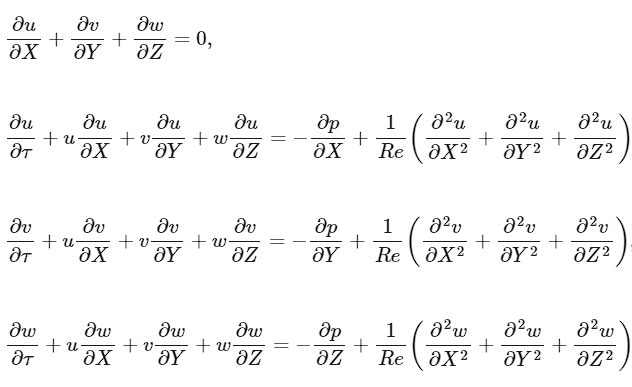
\includegraphics[width=0.8\linewidth, ]{include/nondimeq.png}
\label{Wing motion} 
\caption{Non-dimensionalized governing equations for incompressible flow}
\end{figure}

\section{Overview of FSI}
Fluid Structural Interaction (FSI) is a set of problems within multiphysics modeling where coupling between fluid dynamics and structural mechanics are involved \cite{PEKSEN2018139}. A quantitative understanding of biomechanics present in insects and birds in flight has been a major domain of FSI problems. Such problems are characterized by the action of hydrodynamic forces generated by the fluid over the wing deforming it and the deformed wing in turn affecting the flow. FSI problems are solved using coupled CFD solvers. Similar applications where FSI plays an important role in design considerations include systems like aircraft wings, wind turbine blades, blood flow in the human body, bridges, marine structures, and more.

  \section{Degree of Freedom}
 Degree of freedom refers to the number of possible ways a rigid object can move through space. A body in space has 6 degrees of freedom which corresponds to translation along the x,y, and z axis and rotations around the x,y, and z axis.
 In aerodynamics, the rotation around the x,y, and z axis are 
 called roll, pitch, and yaw motions respectively as shown in Fig.2.2\cite{dof}.

  \begin{figure}[H]
\centering
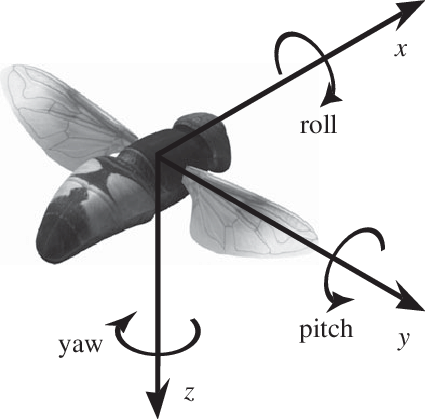
\includegraphics[width=0.5\linewidth, ]{include/yawpitchroll.png}
\label{Wing motion}
\captionsetup{justification=centering}
\caption{Degrees of freedom in rotation}

\end{figure}
 
 \subsection{Euler Angles}
Euler angles include stroke angle $(\psi)$, pitch angle $(\theta)$ and elevation angle $(\phi)$. They are used in flapping kinematics to define the spatial orientation of the wing. Stroke angle also called sweeping angle is defined with respect to the z-axis. The pitch angle is defined with respect to the y-axis. Elevation angle is measured with respect to the x-axis.

\section{Aerodynamic Forces and Moments}

 \subsection{Lift}
Lift is an aerodynamic force produced by the motion of a fluid past an object. Lift acts through the center of pressure of the object and is defined to be perpendicular to the flow direction.

The lift force is defined as:
\begin{equation}
    F_L=0.5*rho*A*C_L*V^2
\end{equation}
where,\\
\nomenclature($rho$)-{Density of fluid} \\ 
\nomenclature{$(A)$}-{Cross sectional area} \\ 
\nomenclature{$(V)$}-{Velocity of the object}\\
\nomenclature{$(C_L)$}-{Coefficient of lift} \\ 


 \subsection{Drag}
Drag is an aerodynamic force produced by the relative motion of an object in a fluid. Drag acts parallel to the flow direction.
\newline

The Drag force is defined as:

\begin{equation}
    F_D=0.5*rho*A*C_D*V^2
\end{equation}

where,\\
\nomenclature{\(rho- \)}{Density of fluid} \\
\nomenclature{\(A- \)}{Cross sectional area} \\ 
\nomenclature{\(V- \)}{Velocity of the object} \\ 
\nomenclature{\(C_D - \)}{Coefficient of drag} \\

 \subsection{Pitching Moment}
The moment (or torque) produced by the lift force on an airfoil if that lift is considered to be applied, not at the center of pressure. The pitching moment is, by convention, considered to be positive when it acts to pitch the airfoil in the nose-up direction. This happens when the center of pressure is ahead of the center of gravity position along the chord line.Aerodynamic forces and pitching moment (negative) in airfoil is shown in Fig.2.3.\cite{pm}

\begin{figure}[H]
\centering
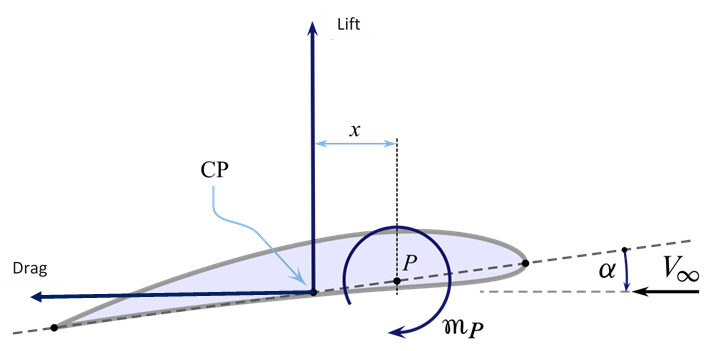
\includegraphics[width=0.7\linewidth, ]{include/forces.png}
\label{forces} 
\captionsetup{justification=centering}
\caption{Aerodynamic forces and pitching moment (negative) in airfoil}
\end{figure}
\subsection{Stroke Moment}
The moment (or torque) produced by the aerodynamic forces on a wing is measured with respect to the z-axis. The pitching moment is, by convention, considered to be positive when it acts counterclockwise.

\subsection{Aerodynamic Work Loop}

The aerodynamic work loop in insect wings describes the energy transfer during flapping flight. As an insect wing oscillates, it undergoes positive and negative work phases, influencing lift and thrust generation. This cyclic process, depicted as a loop, captures the energy expenditure and transfer associated with wing motion. The concept aids in understanding the intricate aerodynamics and power requirements of insect flight, providing insights into the efficiency of their wing movements\cite{workloop,phdthesis}.
Fig.2.4 shows work-loops observed in an insect muscle \cite{loops}

\begin{figure}[H]
\centering
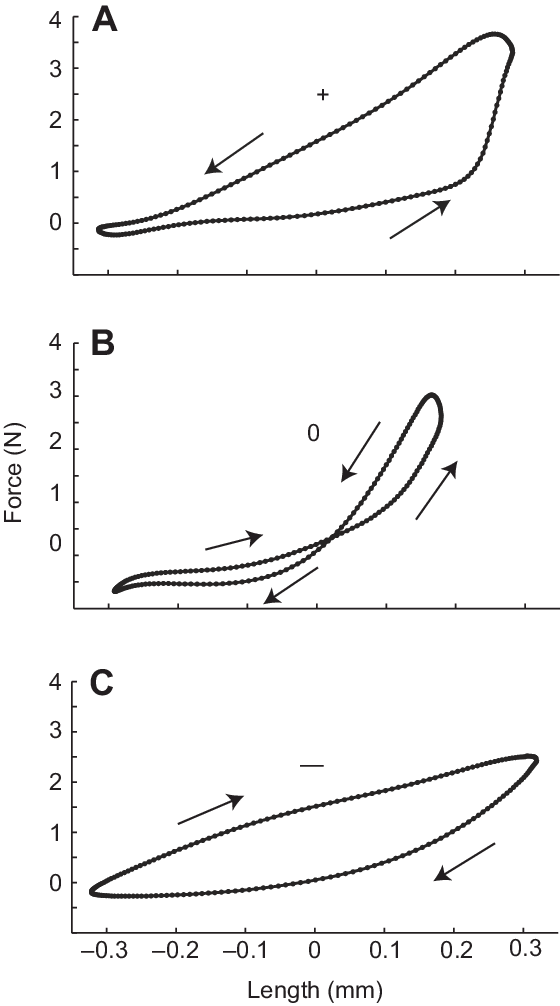
\includegraphics[width=0.6\linewidth, ]{include/Fig2-Example-positive-approximately-zero-and-negative-work-loops-at-A-35C-B.png}
\label{Dynamic stal} 
\captionsetup{justification=centering}
\caption{Work loops: (A) positive work, (B) Near zero work, (c) Negative work}
\end{figure}

\section{Dynamic Stall \& Vortex Shedding}
\subsection{Dynamic Stall}
Dynamic stall is a complex fluid dynamics problem that occurs on an airfoil during rapid, transient motion in which the angle of attack goes beyond the static stall angle. The different stages of stall with variation of angle of attack in an airfoil is shown in Fig.2.5. \cite{SantosPereira2022}.

\subsection{Vortex Shedding}
 Vortex shedding is the periodic shedding of vortices behind an object in a fluid flow, typically occurring when an object obstructs the flow \cite{henne2018dynamic}.
 
\begin{figure}[H]
\centering
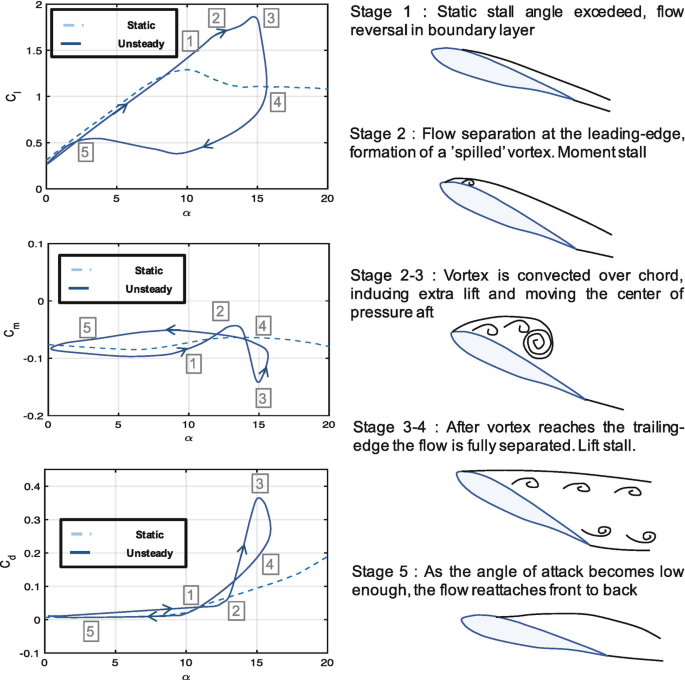
\includegraphics[width=0.9\linewidth, ]{include/460925_1_En_14_Fig1_HTML.png}
\label{Dynamic stal} 
\captionsetup{justification=centering}
\caption{Dynamic stall stages taken from literature}
\end{figure}

 \section{Overset Mesh}
Overset mesh is a method using (at least) two different computational grids, and allowing the grids to overlap and transfer flow field information between the grids. Usually, one mesh describes the whole computational domain (background mesh), and the other mesh describes the mesh for a smaller part of the domain that is moving with a moving object (overset mesh). The background mesh is usually quite coarse while the overset mesh is refined, since the moving object may need a customized refined mesh to predict the more complex flow field around it. An example overset mesh application where it is used to simulate motion of a football is shown in Fig.2.6. \cite{overset}.

\begin{figure}[H]
\centering
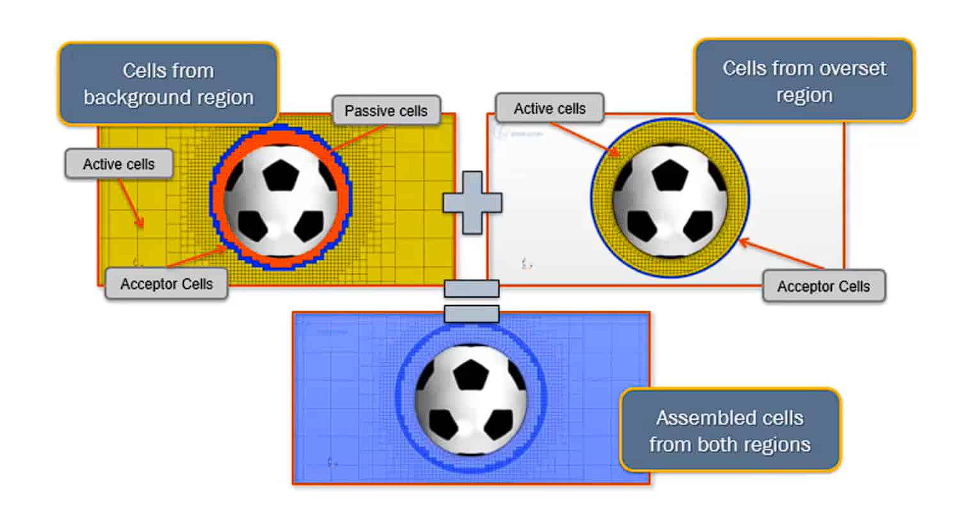
\includegraphics[width=0.7\linewidth, ]{include/overset.png}
\label{overset} 
\captionsetup{justification=centering}
\caption{Overset mesh example from literature: Overset mesh setup for football moving in air}
\end{figure}
 
Overset grids are particularly useful for simulations involving moving components or dynamic interactions. By allowing independent motion of overlapping grids, overset mesh facilitates the simulation of complex fluid-structure interactions, such as rotating or translating components.

\section{Boundary Conditions Used in Simulation}
\subsection{Stagnation Inlet}
The stagnation inlet boundary is an inlet condition that is well-posed for compressible flows, although it is equally valid for incompressible flows. The stagnation conditions refer to the conditions in an imaginary plenum, far upstream, in which the flow is completely at rest. For incompressible flows, Bernoulli's equation is used to relate total pressure, static pressure, and velocity magnitude. Commonly used as the inlet to a simulation of internal flows for which the stagnation conditions are known. 

\subsection{Pressure Outlet}
The pressure outlet boundary is an outflow condition that imposes the working pressure. This boundary pressure can be considered as the static pressure of the environment into which the fluid enters. The working pressure is always expressed relative to the reference pressure. It represents the difference between the absolute pressure and the reference pressure.

\section{$k - \omega$ Turbulence Model}
The $k - \omega$ turbulence model is a two-equation model that solves transport equations for the turbulent kinetic energy k
 and the specific dissipation rate $\omega$
—the dissipation rate per unit turbulent kinetic energy in order to determine the turbulent eddy viscosity.
The standard k−ω model is a low Re model, i.e., it can be used for flows with a low Reynolds number where the boundary layer is relatively thick and the viscous sub-layer can be resolved. Other advantages include a superior performance for complex boundary layer flows under adverse pressure gradients and separations (e.g., external aerodynamics and turbo machinery). 

\section{Drosophila Melanogaster (Fruit Fly)}
 The fruit fly Drosophila Melanogaster is capable of impressive aerial maneuvers, hovering, fast movement, and balancing while moving through the air. This performance is due to a set of muscles, exoskeleton structures, and wings known as the flight motor\cite{Pons_2023} . Studies also found that the number of muscles involved in carrying out such complex motions is significantly low in fruit flies compared to other hovering insects\cite{Lorinda}. The key to understanding how these flies control their flight lies in their complex wing hinge and flight motor. During the flapping motion, fruit flies move their wing at a high angle of attack which causes flow to separate and generate vortices. The difference in the pressure between upper and lower wing surfaces enhanced by the generation of vortices creates the lift force required to hover and fly. Fig.2.7 shows the photograph of a  fruit fly\cite{gompal}.

\begin{figure}[H]
\centering
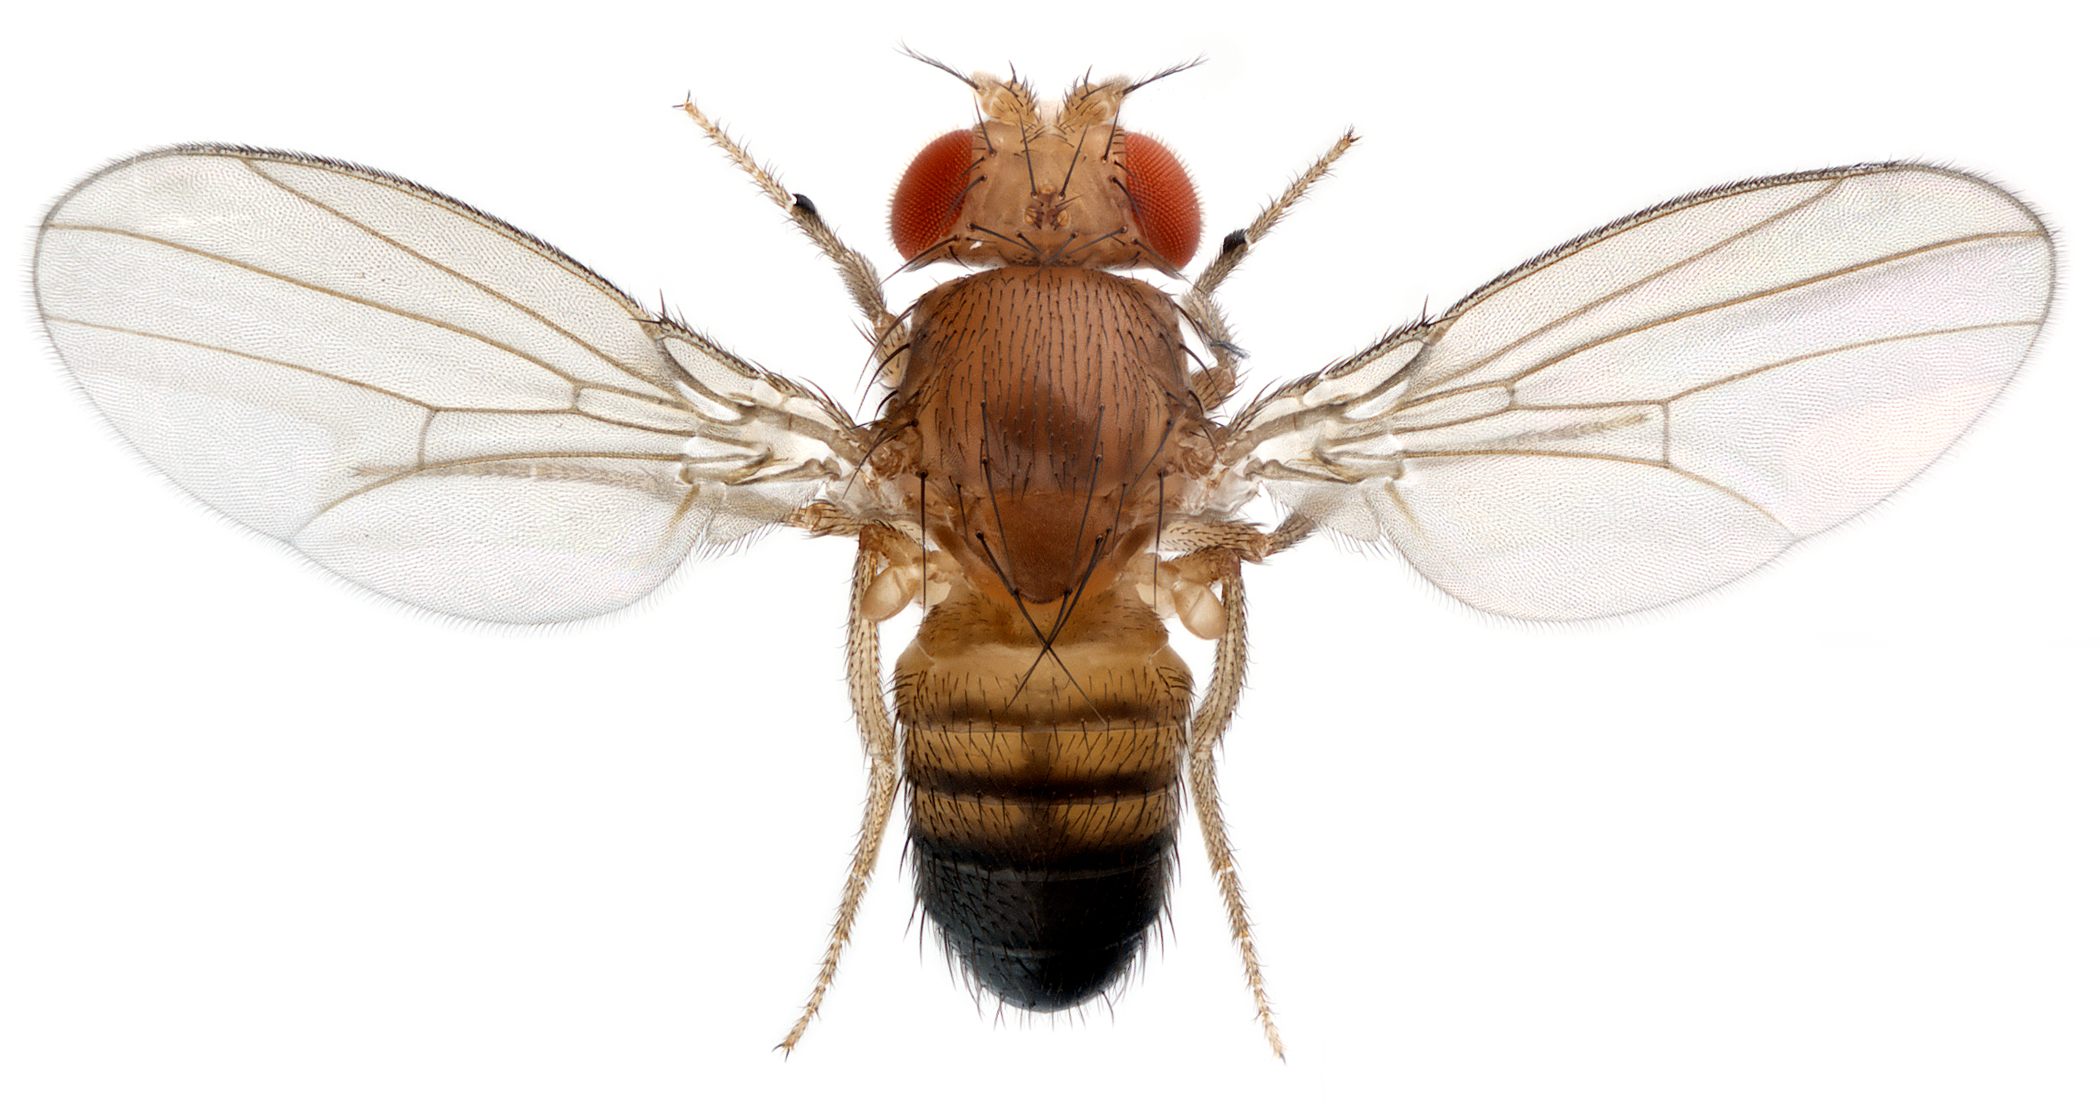
\includegraphics[width=0.6\linewidth, ]{include/MannLoker_composite_fly.png}
\label{Drosophila Melanogaster}
\captionsetup{justification=centering}
\caption{Drosophila Melanogaster (Fruit Fly)}

\end{figure}

 \subsection{Fruit Fly Wing Kinematics}
  The fruit fly kinematics used in the study is taken from literature \cite{kinematics1}. The spatial orientation of the wing defined by Euler angles as well as the translatory position of the wing root in space as a function of time constitutes the wing kinematics discussed in the work. Perl et al\cite{kinematics1} in their work explain the procedure used to record the fruit fly kinematics using high-speed imaging. They observed the kinematics of hovering motion in detail and recorded the trajectories traced by the wing root and wing tip. Maya et al.\cite{kinematics2} in their work did a similar approach recording the kinematics of the fruit fly wing in hovering motion. And utilized a three-dimensional hull reconstruction approach to identify the pose of the fly's body and wings with respect to time. The kinematic data is fitted using Fourier series approximations with 5-8 terms depending on the variable. Wing beat frequency and fluid domain properties are taken from work by Pons et al \cite{Pons_2023}. The fruit fly wing tip and root trajectories plotted using the Fourier series approximations are shown in Fig.2.8. and Fig.2.9.

\begin{figure}[H]
\centering
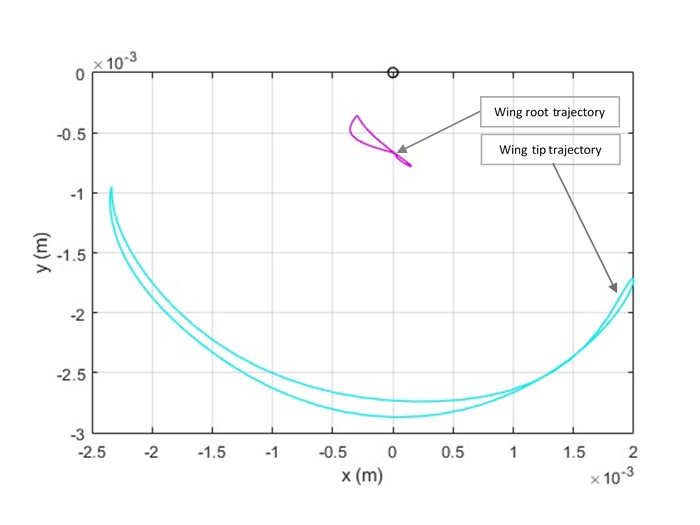
\includegraphics[width=0.99\linewidth, ]{include/roottiptrajectory.png}
\label{Drosophila Melanogaster Wing Trajectory} 
\captionsetup{justification=centering}
\caption{Drosophila Melanogaster Wing Trajectory(top view)}
\end{figure}

\begin{figure}[H]
\centering
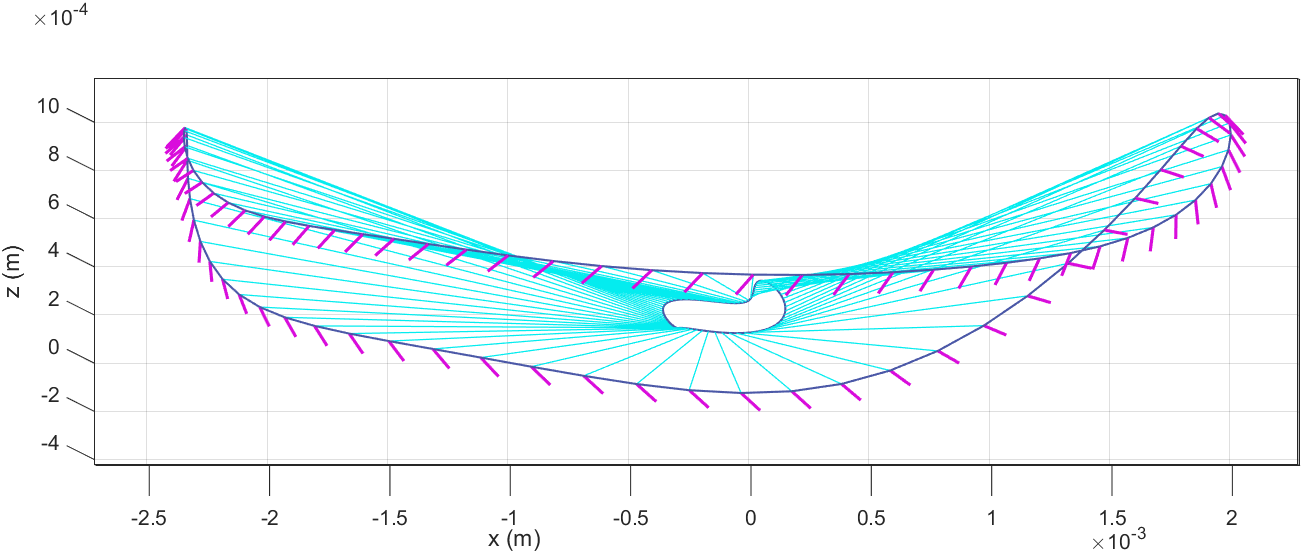
\includegraphics[width=0.99\linewidth, ]{include/untitled1.png}
\label{Drosophila Melanogaster Wing Trajectory}
\captionsetup{justification=centering}
\caption{Drosophila Melanogaster Wing Trajectory (Wing tip view)}
\end{figure}
\vfill



The coefficients of Fourier series approximations used for root trajectory and Euler angle variation for left and right wings are shown below.
\newline

\begin{minted}[frame=single]{matlab}
%Fourier coefficients:
rootCoeffsX = [0.0028929,0.010545,-0.00028184,-0.0008893,
    0.0020166,-0.00069295,0,0,0,0,0,0,0,0,0,0];
    
rootCoeffsY = [-0.0043044,-0.0072242,0.0013097,0.0024587,
    -0.00040197,4.6619e-05,0,0,0,0,0,0,0,0,0,0];
    
rootCoeffsZ = [0.0038606,0.0011476,-0.0010172,0.00095483,
    -0.0012684,-0.00022335,0,0,0,0,0,0,0,0,0,0];
    
phiL_coeff = [  100.8025   73.0880    3.2347   -1.5820   -0.9568   
    4.2585   -0.7202   -1.2631   -0.7062    0.0769    0.4805 ];
    
phiR_coeff = [ -100.8585  -73.8684   -5.1211    0.4147    1.8996 
-3.0560    0.2620    0         0         0         0      ];

psiL_coeff = [ 90.8299    9.3330  -61.6726    2.6201    7.0066 
14.7058   -5.2175   -4.1670   -2.3880    2.0205    6.3990   -0.2757   
-0.6554   -2.0145    0.0945    0.2967   -0.9058 ];

psiR_coeff = [ 89.4874    3.0351  -64.5055    0.0464   -1.3748
14.3808   -8.7732   -0.0201   -5.2505    2.0074    5.6297    0.3232
3.0176   -3.2268    1.1359   -1.8282    0.0011 ];

thetaL_coeff = [ 21.0851    2.1207    1.5256    9.4504    4.3725 
-0.2600   -2.8082    0.4083    1.7483    0         0      ];

thetaR_coeff = [ 18.5406    3.0000    2.9889    6.6285    4.2808 
0.2547   -2.3093    0.0340    1.0105    0         0      ];

\end{minted}

